\pgfplotsset{compat=1.3,width=0.8\columnwidth}
\begin{figure}[H]\centering\vspace{3ex}
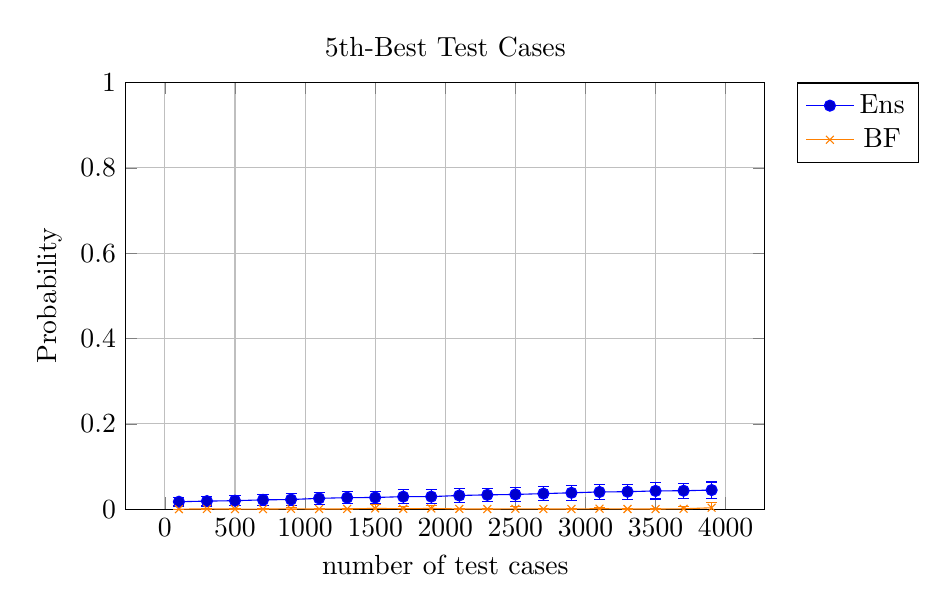
\begin{tikzpicture}
\begin{axis}[width=0.8\columnwidth,height=7cm,
  ymin=0,ymax=1,
  xtick={0,500,1000,1500,2000,2500,3000,3500,4000},
  xticklabels={0,500,1000,1500,2000,2500,3000,3500,4000},
  xlabel={number of test cases},ylabel={Probability},
  title={5th-Best Test Cases},grid=major,
  legend style={at={(1.05,1)},anchor=north west},
  error bars/y dir=both,error bars/y explicit]
\addplot+[mark=*,color=blue,error bars/.cd,y dir=both,y explicit] coordinates {
(100,0.01736000000000001) +- (0,0.010005631067615086)
(300,0.018840000000000013) +- (0,0.01141849555836172)
(500,0.01984000000000001) +- (0,0.012027790948550799)
(700,0.021740000000000002) +- (0,0.01339785240176917)
(900,0.022540000000000004) +- (0,0.014177029423165689)
(1100,0.02528000000000001) +- (0,0.013912320189717603)
(1300,0.026959999999999998) +- (0,0.014176669537788964)
(1500,0.027300000000000012) +- (0,0.014919169971987726)
(1700,0.029300000000000003) +- (0,0.01615770492896278)
(1900,0.029339999999999988) +- (0,0.01616952285590876)
(2100,0.03201999999999998) +- (0,0.016358845825262078)
(2300,0.033499999999999995) +- (0,0.015912067042060267)
(2500,0.03445999999999999) +- (0,0.016161443156412734)
(2700,0.036399999999999995) +- (0,0.016824423451928323)
(2900,0.03833999999999999) +- (0,0.017493567330855764)
(3100,0.040299999999999996) +- (0,0.017967374060007927)
(3300,0.040859999999999994) +- (0,0.01770738344791318)
(3500,0.04275999999999999) +- (0,0.019033332737648494)
(3700,0.04314) +- (0,0.01774077512514084)
(3900,0.044719999999999996) +- (0,0.018882061457848286)
};
\addlegendentry{Ens}
\addplot+[mark=x,color=orange,error bars/.cd,y dir=both,y explicit] coordinates {
(100,0.0) +- (0,0.0)
(300,0.0005800000000000001) +- (0,0.0015919440047582431)
(500,0.00014000000000000001) +- (0,0.0006064281507654607)
(700,0.0002) +- (0,0.0006060915267313264)
(900,0.00068) +- (0,0.002253704433476002)
(1100,0.00024) +- (0,0.0007159979477795239)
(1300,0.0005400000000000001) +- (0,0.0011466010106183494)
(1500,0.0017400000000000002) +- (0,0.00974534949269106)
(1700,0.0008799999999999999) +- (0,0.0052823927787876345)
(1900,0.0016) +- (0,0.0071997732390595166)
(2100,0.0005) +- (0,0.0017053337694733317)
(2300,0.00022000000000000006) +- (0,0.0009100347604933135)
(2500,0.0007400000000000001) +- (0,0.004530216015032521)
(2700,0.00044000000000000007) +- (0,0.0019183326093250876)
(2900,0.00036) +- (0,0.0012577920401745794)
(3100,0.0010400000000000001) +- (0,0.0035911455735756865)
(3300,0.00034) +- (0,0.0017215323027430405)
(3500,0.00024) +- (0,0.0008466018508588031)
(3700,0.0008600000000000001) +- (0,0.004973439658909749)
(3900,0.0032200000000000006) +- (0,0.012822636234409832)
};
\addlegendentry{BF}
\end{axis}
\end{tikzpicture}
\caption{BrokenPeterson (5th)}
\label{fig:BrokenPeterson_(5th)}
\end{figure}
\pgfplotsset{compat=1.3,width=0.8\columnwidth}
\begin{figure}[H]\centering\vspace{3ex}
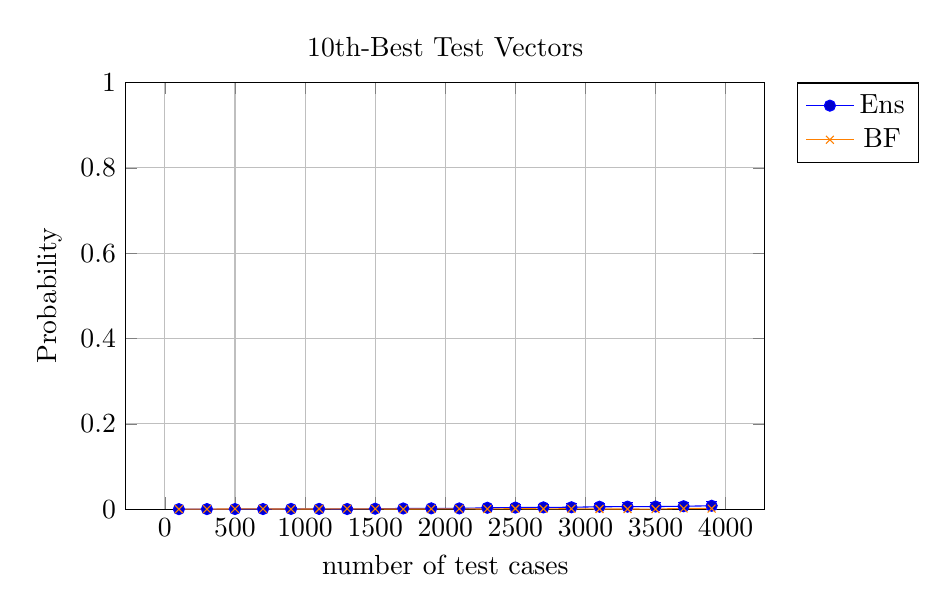
\begin{tikzpicture}
\begin{axis}[width=0.8\columnwidth,height=7cm,
  ymin=0,ymax=1,
  xtick={0,500,1000,1500,2000,2500,3000,3500,4000},
  xticklabels={0,500,1000,1500,2000,2500,3000,3500,4000},
  xlabel={number of test cases},ylabel={Probability},
  title={10th-Best Test Vectors},grid=major,
  legend style={at={(1.05,1)},anchor=north west},
  error bars/y dir=both,error bars/y explicit]
\addplot+[mark=*,color=blue,error bars/.cd,y dir=both,y explicit] coordinates {
(100,4e-05) +- (0,0.000282842712474619)
(300,0.00014000000000000001) +- (0,0.00040456577881446557)
(500,0.00021999999999999998) +- (0,0.0007082603003566023)
(700,0.00028000000000000003) +- (0,0.0008815570640309434)
(900,0.0005800000000000001) +- (0,0.002879129687093314)
(1100,0.0005800000000000002) +- (0,0.0013107094199987536)
(1300,0.0003000000000000001) +- (0,0.0007354021529276429)
(1500,0.0009600000000000003) +- (0,0.0025068070593192975)
(1700,0.00156) +- (0,0.002907836000203869)
(1900,0.0018800000000000004) +- (0,0.004618684325428529)
(2100,0.0016800000000000003) +- (0,0.0032226241050499487)
(2300,0.0032200000000000006) +- (0,0.005346331948740412)
(2500,0.0036200000000000004) +- (0,0.006803030537179435)
(2700,0.004140000000000001) +- (0,0.007392798481478788)
(2900,0.0044) +- (0,0.007835033829029765)
(3100,0.005640000000000002) +- (0,0.0080629158649274)
(3300,0.005860000000000001) +- (0,0.008771498371057786)
(3500,0.006100000000000003) +- (0,0.008493094433787044)
(3700,0.006800000000000003) +- (0,0.009516902257112264)
(3900,0.007900000000000003) +- (0,0.009540996396860124)
};
\addlegendentry{Ens}
\addplot+[mark=x,color=orange,error bars/.cd,y dir=both,y explicit] coordinates {
(100,0.0) +- (0,0.0)
(300,0.0) +- (0,0.0)
(500,0.00062) +- (0,0.0022304936764797893)
(700,0.00068) +- (0,0.0028098950521472563)
(900,2e-05) +- (0,0.00014142135623730954)
(1100,0.00058) +- (0,0.0017389886810019958)
(1300,0.0008) +- (0,0.0034699879432831767)
(1500,0.0006) +- (0,0.002175935173103974)
(1700,0.00018) +- (0,0.0008964783708421275)
(1900,0.0005) +- (0,0.0019086270308410552)
(2100,0.00072) +- (0,0.004384760249885915)
(2300,0.00028000000000000003) +- (0,0.0012128563015309213)
(2500,0.0011800000000000003) +- (0,0.003998418054528005)
(2700,0.00066) +- (0,0.003153294357671426)
(2900,0.0009200000000000001) +- (0,0.00231974664344965)
(3100,0.00034) +- (0,0.0012055991820481226)
(3300,0.00024) +- (0,0.001286666314194023)
(3500,0.00018) +- (0,0.0010038700623291924)
(3700,0.00166) +- (0,0.005783897421959962)
(3900,0.00136) +- (0,0.006579994417217407)
};
\addlegendentry{BF}
\end{axis}
\end{tikzpicture}
\caption{BrokenPeterson (10th)}
\label{fig:BrokenPeterson_(10th)}
\end{figure}
%----------------------------------------
